\documentclass[12pt]{article}

\usepackage[margin=1in]{geometry}
\usepackage{natbib}
\usepackage{tabularx}

\usepackage{Sweave}
\begin{document}



%%% All the primary analysis routines are in mainAnalysis.R



\section{Experiment}
\label{sec:experiment}

\subsection{Participants}

Seventeen native Russian speakers living in or visiting the United
States participated in this experiment at the University of California
at San Diego for cash compensation.  None had arrived in the United
States before age 13, and all reported that they continue to use
Russian on a regular basis and consider it the language they are most
comfortable with.
% 2.2.1. Materials

\subsection{Materials}


Twenty items (listed in full in XXX) were constructed following XXX
pattern.  Each participant saw only one of the four conditions of each
item according to a Latin square design.  These experimental stimuli
were interleaved with 32 items from an unrelated experiment and 52
random fillers such that no two experimental sentences were seen
consecutively.


\subsection{Procedure}
\label{sec:procedure}


Sentences were presented to participants in a non-cumulative
word-by-word moving-window self-paced procedure on a PC laptop
computer running the Linger software \citep{rohde:lingermanual}. Each
trial began with a series of dashes displayed on the computer screen
in place of the words in the sentence. The first press of the space
bar revealed the first word in the sentence, and each subsequent press
of the space bar revealed the next word in the sentence and masked the
previous word. Punctuation was displayed together with the word
preceding it.  The times between button presses were recorded to the
nearest millisecond.  Each sentence was followed by a yes-or-no
comprehension question probing the participant's understanding of the
content of the sentence.  Written instructions in Russian were given
at the outset of the experiment.

\subsection{Data Analysis}
\label{sec:procedure}

Experimental sentences were divided into nine regions of interest as indicated in XXX. Raw reading times were analyzed independently within each region. Prior to analysis, RTs greater than 5000 ms or less than 100ms were excluded. After removing extreme outliers, RTs were further trimmed by removing observations that were more than three standard deviations from a condition mean within a given region. Trials that were incorrectly answered were not excluded from further analysis. This led to a rejection of 108 data points (3.5 \% of the data overall). Response time data were analyzed linear mixed effects (LME) models. The fixed effect structure of all LME models consisted of the experimental factors \textsc{structure}, \textsc{locality}, and their interaction, using simple difference coding (\textsc{structure}: -0.5 for VP attachment,  0.5 for NP attachment;  \textsc{locality}: 0.5 for local attachment, -0.5 for non-local attachment). All mixed effects models used participants and items as random effects, with random intercepts and slopes for all fixed effects (following \cite{barr2013}). In case the model with maximal random effects structure failed to converge, slopes for the interaction term were removed. Accuracy data were analyzed using mixed effects logistic regressions with identical fixed and random effect structure. \textit{p}-values were estimated from model \textit{t}-values by approximation to the standard normal distribution (\cite{baayen2008}).   
  
\subsection{Results}
\label{sec:results}

\subsubsection{Comprehension Accuracy}
\label{sec:acc}

Accuracy on comprehension questions was high, indicating that participants attended to the task. By condition accuracies are provided in \ref{acctable}. Logistic mixed effects modeling of the results indicate no significant differences between conditions. 

% latex table generated in R 2.15.2 by xtable 1.7-0 package
% Thu Aug  1 11:58:08 2013
\begin{table}[ht]
\begin{center}
\begin{tabular}{rll}
  \hline
 & Local & Non-local \\ 
  \hline
NP & 0.94 (0.02) & 0.95 (0.03) \\ 
  VP & 0.96 (0.03) & 0.94 (0.03) \\ 
   \hline
\end{tabular}
\caption{Mean accuracy by condition for Experiment 1. By-participant standard errors in parentheses.}
\end{center}
\end{table}
\subsubsection{Reading Times}
\label{sec:rts}

% latex table generated in R 2.15.2 by xtable 1.7-0 package
% Thu Aug  1 11:58:10 2013
\begin{table}[ht]
\begin{center}
{\scriptsize
\begin{tabularx}{\textwidth}{rlllllllll}
  \hline
 & 1 & 2 & 3 & 4 & 5 & 6 & 7 & 8 & 9 \\ 
  \hline
1 & 637.5 (54) & 704.8 (74) & 856 (108) & 864.6 (93) & 718.6 (64) & 756.6 (59) & 583.6 (52) & 669.6 (53) & 975.9 (84) \\ 
  2 & 618.6 (48) & 725.8 (79) & 891.4 (105) & 861.4 (91) & 677.2 (59) & 721.5 (55) & 578.5 (33) & 667.5 (55) & 975.4 (82) \\ 
  3 & 663.4 (68) & 729.6 (73) & 870.1 (105) & 871.2 (77) & 701.4 (42) & 686.7 (58) & 566.3 (38) & 659.8 (51) & 935.8 (78) \\ 
  4 & 648.5 (62) & 735.1 (89) & 929.5 (130) & 915.1 (107) & 830.3 (80) & 951.4 (96) & 694.6 (58) & 622.9 (42) & 1136.4 (108) \\ 
   \hline
\end{tabularx}
}
\caption{Mean RTs in each region for Experiment 1. By-participant standard errors in parentheses.}
\end{center}
\end{table}
Mean RTs in each region, along with by-participant standard error, is presented in \ref{rttable} and in \ref{rtfig}. Prior to the critical relative pronoun region, no significant effects of any experimental fixed effects were found. In the region immediately following the relative pronoun (region 6), mixed effects modeling showed a significant effect of \textsc{locality} ($\beta$ = -121 ($\pm$ 53), $p <$ 0.05), and a significant interaction of \textsc{locality} and \textsc{structure} ($\beta$ = 298 ($\pm$ 112), $p <$ 0.01). In region 7, there was a marginal effect of \textsc{locality} ($\beta$ = -62 ($\pm$ 34), $p <$ 0.1), as well as a marginal interaction \textsc{locality} and \textsc{structure} ($\beta$ = 129 ($\pm$ 66), $p <$ 0.1). Additional, in region 9 there was a significant interaction of \textsc{locality} and \textsc{structure} ($\beta$ = 253 ($\pm$ 120), $p <$ 0.05), as well as a marginal effect of \textsc{locality} ($\beta$ = -127 ($\pm$ 77), $p <$ 0.1).

The critical interaction at region 6 was resolved by fitting a second LME model that used nested contrasts to estimate the effect of \textsc{locality} within each level of the \textsc{structure} factor. The results of this model indicate a significant effect of locality for VP attachment conditions ($\beta$ = -270 ($\pm$ 91), $p <$ 0.01). There was no significant effect of locality for NP attachment conditions ($\beta$ = 28 ($\pm$ 61), $p =$ 0.646).


\begin{figure}
\begin{center}
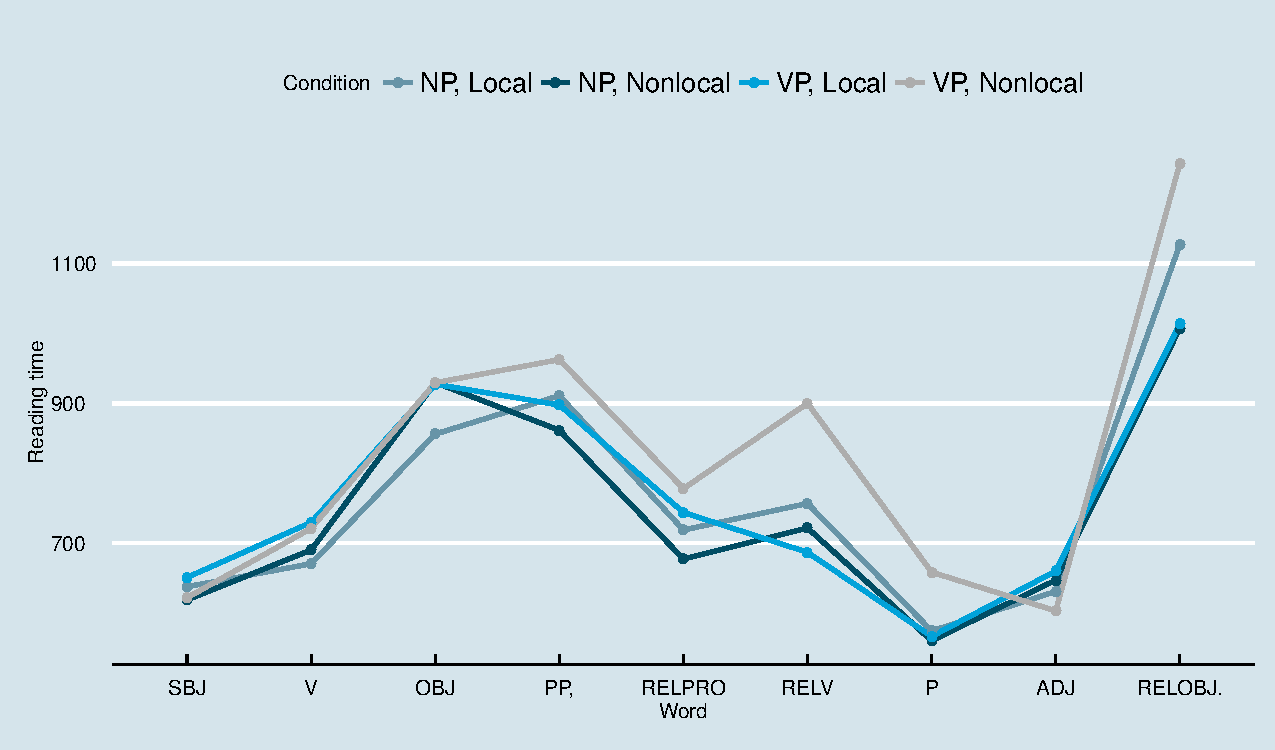
\includegraphics{russian-extraposed-rcs-mainplot}
\end{center}
\caption{Mean reading times in Experiment 1. Error bars represent standard error by participants.}
\label{rtfig}
\end{figure}

\bibliographystyle{apalike}
\bibliography{russian-extraposed-rcs}




\end{document}

%%% Local Variables: 
%%% mode: latex
%%% TeX-master: t
%%% End: 
